%!TEX root = thesis.tex
\chapter{Model implementation}\label{chap:methods}
\thispagestyle{plain}

This chapter describes the model implementation process, including the underlying theory.
The first section explains the general concepts of glacier volume/area scaling relations as well as the theoretical basis for the implemented temperature-index mass balance model and glacier evolution model. Programming related implementation details are shown in the second section, including the description of relevant classes and methods, which serves as documentation. The third and final section of this chapter details the experimental setup for the following model evaluation.

% ==== SECTION 1 ===============================================================
\section{General concepts} % (fold)
\label{sec:general_concepts}

    Before starting to write any code, a solid theoretical foundation has to be established. A summary of the extensive work on \vas{} \citep{Bahr1997, Bahr1997a, Bahr1997b, Bahr2015} is provided,  including a discussion about the ill-posed nature of ice volume inversions \citep{Bahr2014}. The description of the implemented mass balance model and glacier evolution model follows \citet{Marzeion2012b}.

    \subsection{Glacier volume/area scaling} % (fold)
    \label{sub:glacier_volume_area_scaling}

        \begin{tldrbox}[Glacier \vas{}]{tldr:glacier_vas}
            \item \Vas{} relates a glacier's ice volume $V$ to its surface area $A$ via the power law $V=cA^\gamma$. It has a solid physical basis, the derivation does not rely on any simplifications.
            \item Two separate derivations and three different choices of a single closure condition all result in the same value for the scaling exponent $\gamma_\text{glacier} = 1.375$, which implies self consistency. The scaling constant $c$ is a random variable that varies from glacier to glacier.
            \item Response time scaling should be used in conjuncture with \vas{} to simulate transient glaciers.
            \item Scaling relations are determined, validated and should therefore be applied solely to large samples of glaciers spanning a large range of sizes, and not on single glaciers, parts or individual branches of glaciers, or glacier complexes spanning over flow divides.
        \end{tldrbox}

        % Overview
        Ice volume is one of the most fundamental geometric glacier properties and yet unknown for the vast majority of all of the world's glaciers and ice caps. Direct measurements of ice volume and ice thickness (or any other internal property such subsurface topography, internal velocities, sliding rates, etc.) are difficult to obtain, incident to time and cost extensive fieldwork. Hence, glacier internal properties are often inferred from surface properties, a process called inversion \citep{Bahr2014}. \Vas{} has been, and still is, one of the most commonly used ice volume inversion methods.

        A glacier's ice volume $V$ can be estimated from its surface area $A$ using the power law $V = c\, A^\gamma$. Hereby, the scaling constant $c$ is a random variable, changing from glacier to glacier. The scaling exponent $\gamma$ is a constant for a given geometric class of glaciers: it is distinguished between valley glaciers $\gamma_\text{glacier} = 1.375$, and radially symmetric ice caps $\gamma_\text{ice\ cap} = 1.25$\footnote{The following section focuses on mountain glaciers, however the general concepts hold also true for ice caps with The different values for scaling exponent and scaling constant result from different closure conditions (e.g., radial symmetric shape). A detailed derivation can be found in \citet[][Section 7.2]{Bahr2015}.}. The scaling parameters were initially determined empirically by computing a linear regression between $V$ and $A$ measurements in log-log space \citep[e.g.,][]{Chen1990}. The underlying theoretical principles were established later by \citet{Bahr1997, Bahr1997b}. The following basic derivation relies on simple geometric observations, following \citet{Bahr1997b, Bahr2015}.
        
        \subsubsection{Basic derivation} % (fold)
        \label{ssub:basic_derivation}

            Glacier volume can be scaled with a number of quantities (e.g., area, thickness, length and velocity), of which surface area is the most easily measurable one. To obtain a volume quantity $V$ of dimension $\mathrm{L}^3$ (hereby $\mathrm{L}$ represent the fundamental dimension of length), an area $A$ of dimension $\mathrm{L}^2$ must be multiplied by one additional quantity of dimension $\mathrm{L}$. In the specific case of glacier ice volume and glacier surface area, the average ice thickness $\bar{h}$ is an obvious choice. Thereby, $\bar{h}$ can be estimated as the centerline thickness $h$ corrected by shape factor, to account for lateral drag and non U-shaped bed cross sections. This shape factor $F$ scales as ratio of width to thickness $F\propto w/h$. The surface area is a product of average length $\bar l$ and average width $\bar w$. Observations suggest that $w\propto l^q$, with $q\approx 0.6$ for valley glaciers. It is sensible to use the average values as characteristic values. By bringing all those relations together, it can be shown that glacier volume scales with surface area as
            \begin{align}
            \begin{split}
                V &\propto A\cdot \bar{h} = A\cdot Fh \\
                    &\propto \bar w\bar l\cdot \frac{\bar w}{h}h = \bar w^2\bar l \\
                    &\propto \bar l^{2q+1} \\
                    &\propto A^\frac{2q+1}{q+1} = A^\gamma = A^{1.375}
            \end{split}
            \end{align}
            The scaling relations for $F$ and the $w$ are necessary to fully express $V$ as a function of $l$ and consequentially of $A$. Those so called closure conditions are hypothesized but backed by observational data, and the \textit{universal} nature of the scaling exponent stands and falls with them. However, the same \vas{} relation can be derived via two independent and mathematically consistent pathways. The following section gives a brief overview over the derivation from a dimensional analysis and the physical reasoning behind glacier scaling relations, following \citet[Section 4 - 7]{Bahr2015}.
        
        % subsubsection basic_derivation (end)
        
        \subsubsection{Formal derivation} % (fold)
        \label{ssub:formal_derivation}

            % Dimensional analysis
            Glacier \vas{} can be derived from a dimensional analysis of the full set of continuum equations \citep{Bahr1997b, Bahr2015}. The set of continuum equations describing the ice flow of glaciers accounts for mass balance and mass conservation via the continuity equation, and force balance and momentum conservation via the equation of motion. Both equations are linked by the constitutive equation, relating force to deformation, or more precisely stresses to strain rates \citep[e.g.,][]{CuffeyPaterson2010}. The values of variables like glacier geometries, surface mass balance, sliding velocity, and others are defined by boundary conditions. Since those boundary conditions affect only the values but not the dimensions of the relevant variables, they have no effect on the dimensional analysis. Similarly, the inclusion of an energy conservation equation only adds additional non-dimensional parameters. This does not alter other scaling relations and is therefore omitted \citep{Bahr2015}. The full set of continuum equations consist of eighteen fundamental variables, which span over the three fundamental dimensions length $\mathrm{L}$, mass $\mathrm{M}$, and time $\mathrm{T}$. According to the Buckingham Pi theorem \citep[e.g.,][]{Evans1972, Yarin2012} this yields a set of fifteen dimensionless $\Pi$-groups. The $\Pi$-groups relevant for \vas{} are listed below, taken from \citet[Section 4.1, Eq. 26, 28 \& 33]{Bahr2015}:
            % \begin{align}
            %     \Pi_2 &= \frac{x}{z} \\
            %     \Pi_4 &= \frac{u_x}{u_z} \\
            %     \Pi_9 &= \frac{A\rho^n{g_x}^nz^{n+1}}{u_x}
            % \end{align}
            \begin{align}
                \Pi_2 = \frac{x}{z}, \qquad\qquad
                \Pi_4 = \frac{u_x}{u_z}, \qquad\qquad
                \Pi_9 = \frac{A\rho^n{g_x}^nz^{n+1}}{u_x}.
            \end{align}
            Hereby, $x$ and $z$ represent length and height (or more formally, distance in longitudinal and vertical direction), $u_x$ and $u_z$ velocities in $x$ and $z$ direction, $\rho$ the ice density, $g_x$ the gravitational acceleration in $x$ direction, and $n$ the exponent of Glen's flow law \citep[e.g.,][Chapter 3.4.4]{CuffeyPaterson2010}. The number indices are arbitrary.
            % Stretching transformation
            The same set of dimensionless parameters can be computed from a stretching analysis, with the added benefit of knowing the respective physical origin and removing potential mathematical ambiguities \citep[Section 5]{Bahr2015}. The stretching analysis shows that the geometric similarity $\Pi_2$ and the kinematic similarity $\Pi_4$ follow from the constitutive equation, while the velocity relationship $\Pi_9$ follows from a combination of the constitutive equation and the equation of motion \citep[Section 6]{Bahr2015}.

            Choosing and combining the $\Pi$-groups most relevant to the problem influences the form of the scaling constant $c$. The dimensionless parameters may vary from glacier to glacier, and so does $c$. However,  variations in $c$ are several orders of magnitude smaller than variations in $A$ and $V$. This explains the strong power law relation between $A$ and $V$, undeterred by variations in $c$, and allowed the empirical estimation in the first place \citep{Bahr2015}. Combining the above shown $\Pi$-groups yields
            \begin{align}\label{eq:pi_groups_combi}
                \frac{\Pi_4 \Pi_9}{\Pi_2} = \frac{A\rho^n{g_x}^nz^{n+2}}{u_z x}.
            \end{align}
            The characteristic values cancel when solving for area and volume, which is why their exact choice is of secondary importance. However, the choice will influence the scaling exponent $\gamma$. Some choices make intuitive sense, like using glacier length as characteristic length $l \equiv x$, average thickness as characteristic thickness $h \equiv z$ and average width as characteristic width $w \equiv y$. Other choices are motivated by known closure conditions, like using the mass balance at the glacier terminus as characteristic vertical velocity $\dot b \equiv u_z$ \citep{Bahr2015}. Closure conditions are additional scaling relations backed by observations. They are necessary to express the ice thickness purely as function of glacier length. The following closure conditions are used:
            \begin{itemize}
                \item The \vas{} relation encapsulates the erosive power of a glacier by relating the ``superficial'' glacier size to its geometry. Similarly, a glacier's width relates to its length. Observational data suggests that the average glacier width scales with glacier length as $w=c_q\, l^q$ with $q\approx 0.6$ for valley glaciers. Hereby, $c_q$ is a variable scaling constant \citep{Bahr1997a, Bahr2015}.
                \item Longer glaciers tend to span over a wider range of elevations and reach further into the ablation zone. The magnitude of the (point) mass balance is higher at lower---and thereby warmer---elevations. Hence, the mass balance scales with glacier length as $\dot b = c_m\, l^m$. Hereby observations suggest $m\approx 2$ for valley glaciers, while $c_m$ is a variable scaling constant \citep{Bahr1997b, Bahr2015}.
            \end{itemize}
            Substituting characteristic values and the mass balance closure into Equation~\ref{eq:pi_groups_combi}, and solving for $h$ yields
            \begin{align}\label{eq:h_fct_pigroups}
                h = \left(\frac{\Pi_4 \Pi_9 c_m}{\Pi_2 A\rho^n {g_x}^n}\right)^\frac{1}{n+2}\, l^\frac{m+1}{n+2}.
            \end{align}
            Using $V = lwh$ and $S=lw$, substituting Equation~\ref{eq:h_fct_pigroups} and the width closure, and combining the two yields
            \begin{align}\label{eq:vas_exponent}
                V &= c_A\, S^{1+\frac{m+1}{(n+2)(q+1)}}\\
                  &= c_A\, S^\gamma.
            \end{align}
            While the scaling constant $c_A$ depends on a bunch of dimensionless parameters and other constants (not shown), the scaling exponent depends only the mass balance scaling exponent $m$, the exponent of Glen's flow law $n$ and the width scaling exponent $q$. With the values suggested above this results in
            \begin{align}
                \gamma &= 1 + \frac{m+1}{(n+2)(q+1)}\\
                       &= 1 + \frac{2+1}{(3+2)(0.6+1)}\\ 
                       &= 1.375.
            \end{align}
            It can be shown that the used closure conditions are not independent of each other and only one closure condition is strictly necessary. Additionally, using independent observational data for all three closure conditions results in the same value for $\gamma$.            
        
        % subsubsection formal_derivation (end)

        \subsubsection{Usage and best practice} % (fold)
        \label{ssub:usage_and_best_practice}

            Besides showing an improved and more detailed derivation, \citet{Bahr2015} review the usage of \vas{} in thirty-three papers published between 2006 and 2014. While all studies provide new insights, certain misconceptions in the validity and applicability of \vas{} led to a few unsuccessful applications. \citet[Section 8]{Bahr2015} address all particular characteristics of \vas{} that have been ground for misunderstandings. The suggested guidelines for practical applications are summarized below:
            \begin{itemize}
                \item Fix the scaling exponent $\gamma$ to its physically based value, and let the scaling constant $c$ vary as necessary in time, space and others.
                \item Apply \vas{} to large populations of glaciers, whereby the aggregate volume gives the most accurate estimate. Avoid applying \vas{} to single glaciers and treat the result as order of magnitude estimate if you do.
                \item Avoid applying \vas{} to fractional parts of glaciers and glacier complexes that span over flow divides.
                \item Use response time scaling in conjuncture with \vas{} to account for transient glacier states.
            \end{itemize}
            
        % subsubsection  (end)

        % \subsubsection{Glacier volume estimation as ill-posed problem} % (fold)
        % \label{ssub:glacier_volume_estimation_as_ill_posed_problem}

        %     \Vas{} shares an inherent problem with all methods of ice volume (or ice thickness) inversion. The unbalanced application of boundary conditions typical for inversions (all on the surface, none on the bottom) results in an ill-posed problem, the type of numerical approach is thereby irrelevant. A problem is defined as \emph{ill-posed} if the solution is either not unique, not stable or does not exist \citep{Zhdanov2002}. Given that every glacier has a volume, a solution must exist. This leaves us with either unstable and/or non-unique solutions. Both cases imply the existence of a cloud of possible solutions \citep{Bahr2014}.

        %     However, the ill-posed nature of the problem agrees with our understanding of glaciers. On one hand, glaciers with similar surface areas can have vastly different ice volumes, based on their geographic location, climatic conditions, or other local characteristics (i.e., non-unique solutions). On the other hand, given a glacier's tendency to smooth out small scale basal features, similar surface topographies can arise from vastly different basal topographies. In other words, small changes in surface topography are most likely caused by substantially different conditions in bed topography (i.e., unstable solutions). While the problem of ice thickness inversion is and will be ill-posed by definition, there are mitigation factors that render \vas{} and other numerical approaches useful nonetheless. Some of those factors are listed below, without going into much detail. For a full discussion of the topic see \citet{Bahr2014}.

        %     Ill-posed problems are not unsolvable. The inversion can be constrained by so called regularization processes. Thereby, reasonable bounds are placed on the solution by assuming parts of it. Additionally, the sum over a substantially large set of glacier volumes will be a good estimate. Random errors of individual glaciers are likely to balance each other, according to the law of large numbers. However, uncertainties introduced by other parameters (e.g., Glen's A-parameter, sliding parameters, ...) must be addressed separately \citep{Bahr2014}.

        %     No matter the type of inversion, errors in surface measurements (or calculations) grow chaotically and exponentially with depth \citep{Bahr1994}. The instabilities depends on the spatial resolution, or more precisely the spatial wavelengths and associated frequencies. Thereby, higher frequencies result in a stronger exponential growth. Limiting unstable short wavelengths or using only substantially large spatial wavelengths can produce stable solutions \citep{Bahr2014}. Herein lies the inherent advantage of \vas{}, since the shortest length scales used in the scaling relations are already in the order of the entire glacier length. However, also other numerical approaches can produces stable results by explicitly filtering the correct wavelengths. And no approach, neither \vas{} nor any numerical model, is able to produce unique solutions.

        %     % subsubsection glacier_volume_estimation_as_ill_posed_problem (end)

    % subsection glacier_volume_area_scaling (end)

    \subsection{Temperature index model} % (fold)
    \label{sub:temperature_index_model}

        % \begin{tldrbox}[Temperature index model]{tldr:temperature_index_model}
        %     \item The temperature index model computes the yearly specific mass balance with solid precipitation and positive melting temperature as input, depending on the glacier specific temperature sensitivity \mustar{}.
        %     \item The temperature sensitivity \mustar{} relates the melting temperature to the actual ice loss and needs to calibrated for each glacier.
        %     \item ... calibration %TODO
        %     \item The \vas{} model estimated a glacier-wide average mass balance values, while the flowline model computes point mass balance values for each elevation band.
        % \end{tldrbox}

        A glacier's annual specific surface mass balance $B$ is the area-averaged difference between accumulation and ablation over the course of a year. Hereby, accumulation refers to mass gain via snowfall, avalanches, snow drift, etc., while ablation refers to mass loss via ice melt, sublimation, calving, etc. The temperature index mass balance model explained and implemented hereafter relies solely on two input parameters: the area-averaged monthly solid precipitation onto the glacier surface $P_i^\text{solid}$ and the monthly mean air temperature at the glacier's terminus elevation $T_i^\text{terminus}$. Hereby, the index $i$ denotes the month of the year. The mass balance equation described by \citet{Marzeion2012b} reads
        \begin{align}
            \label{eq:mass-balance}
            B = \left[\sum_{i=1}^{12}\left[
                    P_i^\text{solid}  - \mu^* \cdot \max\left(T_{i}^\text{terminus} - T_\text{melt},\ 0\right)
                \right]\right] - \beta^*.
        \end{align}
        The terminus temperature $T_{i}^\text{terminus}$ is computed by scaling the monthly mean air temperature $T_i$ from the climate date reference elevation $z_\text{ref}$ to the glacier's terminus elevation $z_\text{min}$ using the temperature lapse rate $\gamma_\text{temp}$.
        \begin{align}
            T_i^\text{terminus} = T_i \cdot \gamma_\text{temp} (z_\text{min} - z_\text{ref})
        \end{align}
        The temperature at the maximum glacier elevation $T_{i}^\text{max}$ is computed analogously $T_{i}^\text{max} = T_i \cdot \gamma_\text{temp} (z_\text{max} - z_\text{ref})$, whereby $z_\text{max}$ represent the maximum glacier surface elevation. The positive melting temperature is computed as the difference between $T_{i}^\text{terminus}$ and temperature threshold for ice melt $T_\text{melt}$, with an obvious lower bound of \SI{0}{\celsius}. The glacier's temperature sensitivity \mustar{} relates the positive melting temperature to the actual ice loss and needs to be calibrated for each glacier (as does the mass balance residual \bias{}). The \hyperref[ssub:mb_calib]{calibration process} of these mass balance parameters is described below.
        
        The area-average monthly solid precipitation onto the glacier surface $P_i^\text{solid}$ is computed from the total precipitation of the climate data $P_i$ as
        \begin{align}\label{eq:solid-precip}
            P_i^\text{solid} = P_i \cdot f_\text{solid} \cdot (1 + \gamma_\text{precip} \cdot (z_\text{mean} - z_\text{ref})).
        \end{align}
        Hereby, $P_i$ is scaled from $z_\text{ref}$ to the average glacier surface elevation $z_\text{mean}$ using the precipitation lapse rate $\gamma_\text{precip}$ (given in units of percentage of precipitation per meters of elevation change [\si{\percent\per\meter}]). The fraction of solid precipitation $f_\text{solid}$ depends on the 
        relation of $T_i^\text{terminus}$ and $T_{i}^\text{max}$ to the temperature thresholds for solid and liquid precipitation, $T^\text{solid}$ and $T^\text{liquid}$, respectively. The fraction of solid precipitation is linearly interpolated ($f_\text{solid} = 1 + \frac{T_{i}^\text{terminus} - T^\text{solid}}{\gamma_\text{temp}\cdot(z_\text{max} - z_\text{min})}$) between the two extreme cases of only solid ($T_i^\text{terminus} < T^\text{solid} \ \Rightarrow f_\text{solid} = 1$) and only liquid precipitation ($T_i^\text{max} > T^\text{liquid} \Rightarrow f_\text{solid} = 0$). Values for the temperature thresholds are discussed below.

        % Old version... I'll keep it for a while in case I need it...
        % For terminus temperatures below the threshold for solid precipitation, all precipitation is solid ($T_i^\text{terminus} < T^\text{solid} \ \Rightarrow f_\text{solid} = 1$). For temperatures at the maximum glacier surface elevation above the threshold for liquid precipitation, all precipitation is liquid ($T_i^\text{max} > T^\text{liquid} \Rightarrow f_\text{solid} = 0$). And for temperatures in between, the fraction of solid precipitation is interpolated linearly between 0 and 1 as $f_\text{solid} = 1 + \frac{T_{i}^\text{terminus} - T^\text{solid}}{\gamma_\text{temp}\cdot(z_\text{max} - z_\text{min})}$.
        
        The downscaling of GCM data for the use with glacier mass balance models requires one additional step. The monthly precipitation amount is scaled by an additional factor $a$, since precipitation in mountainous regions is generally underestimated. While this scaling factor is implemented in the mass balance models (as \lstinline`prcp_scaling_factor`), it is not a physical component of the  mass balance equation and therefore omitted in Equation~\ref{eq:solid-precip}. Values of $a$ are discussed below.

        % Keepf for xval discussion section.
        % A global mean of $a = 2.5$ is found by \citet{Giesen2012}, whereas \citet{Marzeion2012c} found a mean of 2.1 for Central Europe and Scandinavia. The sensitivity study conducted by \citet[Section 2.2.2, Figure 4]{Marzeion2012b} shows the strongest correlation between observed and modeled mass balance for $a \approx 1.3$ and the highest skill score for $a \approx 2.5$. Since the variability of the modeled mass balance is quite low for values of $a \leq 2.5$, this is the used factor.

        The values of the above mentioned hyper parameters, like temperature thresholds, lapse rates, and scaling factors, can and should be calibrated depending on the region and the used baseline climate. The OGGM ships with default global values based on climate data provided by the Climate Research Unit \citep[CRU,][]{Harris2014} and default Alpine values based on the Historical Instrumental Climatological Surface Time Series Of The Greater Alpine Region \citep[HISTALP, ][]{Auer2007}. These default values result from a leave-one-glacier-out cross validation between all reference glaciers. Thereby, individual hyper parameters are iteratively changed within a given range, as originally proposed by \citet{Marzeion2012b} and refined for regional use by \citet{Dusch2018}. An analogous cross validation is performed for the \vas{} model using HISTALP data as baseline climate. The following parameters are chosen based on a simple scoring function of the computed statistical measures and used for all runs on Alpine glaciers: $a = 2.5, T^\text{melt} = \SI{-0.5}{\celsius}, T^\text{solid precip} = \SI{2.0}{\celsius}$. The flowline mode uses the default OGGM HISTALP parameters ($a = 1.75$, $T^\text{melt} = \SI{-1.75}{\celsius}$, $T^\text{solid precip} = \SI{2.0}{\celsius}$, \citet{Dusch2018}) for the same runs. The 21st century projections are based on CRU climate data and the latest data from the Coupled Model Intercomparison Project \citep[CMIP6, ][]{Eyring2016_CMIP}. Hence the \vas{} model uses updated global parameters taken from \citet{Malles2020} for those runs, while the flowline model falls back to the OGGM default values. However, differences between those values are of minor importance, since the temperature sensitivity \mustar{} compensates for most systematic biases in the climate input data \citep[Appendix A]{Maussion2019}.

        \subsubsection{Calibration of the mass balance parameters} % fold
        \label{ssub:mb_calib}

            A complete and thorough description of the mass balance calibration process for this particular temperature index model can be found in \citet[Section 2.1.9-10]{Marzeion2012b} and \citet[][Section 3.3]{Maussion2019}. The following summary is included here for completeness.
            
            The first step is to estimate the so called $\mu(t)$ \emph{candidates} for all glaciers with available mass balance records (254 glaciers globally, see \citet{WGMS2017}). This is done by requiring the average mass balance $\overline B(t)$ over the 31-year period centered around the year $t$ to be zero and solving for $\mu(t)$.
            \begin{align}\label{eq:mu-candidates}
                \mu(t) = \frac{P_\text{clim}^\text{solid}(t)}{\max(T_\text{clim}^\text{terminus(t)} - T_\text{melt}\, 0)},
            \end{align}
            whereby $P_{\text{clim}}^{\text{solid}}(t)$ and $T_{\text{clim}}^{\text{terminus}}(t)$ are the average yearly solid precipitation amount and average yearly air temperature at the glaciers terminus during the climatological period centered around the year $t$, respectively. The next step is to solve the mass balance equation (Equation~\ref{eq:mass-balance}) for each $\mu(t)$ candidate and compare the results to the mass balance observations. The computed difference $\beta(t)$ is a measure of how good the temperature sensitivity candidate approximates the \textit{real} value, denoted as \mustar{}. Hence, \mustar{} is chosen as the candidate $\mu(t = t^*)$ for which the absolute bias is minimal $\beta^* \coloneqq \beta(t = t^*) \approx 0$---which in the best case is around zero. Hereby, the \textit{equilibrium year} \tstar{} represents the center of the 31-year climatic period where the given glacier geometry would stay in equilibrium. However, this is more of a model parameter and should not be overinterpreted as a real world value. The same is true for the corresponding temperature sensitivity \mustar{} and mass balance residual \bias{}.

            For all glaciers without mass balance records, \tstar{} and \bias{} are interpolated from the ten closest glaciers, inversely weighted with distance. The temperature sensitivity is computed by requiring the mass balance to be zero ($\overline B(t^*) = 0$) and solving for \mustar{}. The temperature sensitivity \mustar{} depends highly on glacier specific factors, such as avalanches from surrounding terrain, topographical shading, etc. Therefore, \mustar{} can vary drastically from one glacier to another, even between neighboring glaciers. By contrast, it is intuitively more likely for a glacier to be in equilibrium if its surrounding glaciers are in equilibrium as well. This is one major factor, why the interpolation of \tstar{} instead of \mustar{} reduces the mass balance error in a leave-one-out cross validation \citep[cf.][]{Marzeion2012b, Maussion2019}.

        % subsubsection mb_calib (end) 


        \subsubsection{Implementation note} % (fold)
        \label{ssub:mb_calib_implementation_note}

            The results of the calibration steps outlined above depend on the glacier outlines, the climate data, and the mass balance hyper parameters (i.e., the temperature thresholds, lapse rates and the precipitation scaling factor). The equilibrium year \tstar{} and mass balance residual \bias{} computed for each reference glacier are stored in the \lstinline`ref_tstars.csv` file. Hence, for a given combination of RGI version, baseline climate and hyper parameters the calibration for the reference glaciers has to be done only once. Afterwards, the results can be read directly from the corresponding file. The OGGM comes with reference tables for combinations of RGI version 5 and 6, and CRU version 4 and HISTALP. The \vas{} model provides its own reference tables, for CRU version 4 and HISTALP data but only for RGI version 6, using the hyper parameters detailed in Section~\ref{sub:temperature_index_model}.
        
        % subsubsection mb_calib_implementation_note (end) 

        \subsubsection{Differences in mass balance model between the scaling and flowline model}

            The \vas{} mass balance model computes an average mass balance value for the entire glacier. The mass balance model requires only the minimal and maximal glacier elevation as additional input parameters ($z_\text{min}$, $z_\text{max}$), to compute the monthly terminus temperature $T_i^\text{terminus}$ and the area averaged monthly amount of solid precipitation $P_i^\text{solid}$. The flowline model requires a mass balance value for each grid point of the flowline (i.e., for each elevation band). Therefore, the mass balance is computed as a function of elevation $B(z)$. Hence, the elevation of the grid points must be supplied as input parameters. Solid precipitation and air temperature are then computed for the given points of elevation, resulting in a point mass balance estimate.
    
    % subsection temperature_index_model (end)

    \subsection{Glacier evolution model} % (fold)
    \label{sub:glacier_evolution_model}

        % Volume/area scaling must be used in conjuncture with proper response time scaling (Bahr, 2015)
        The \vas{} relation is derived from the complete set of continuum equations, without any assumptions of plane strain, shallow ice, perfect plasticity, or steady state conditions. This derivation from the fully time dependent equation of motion allows the volume $V$, area $A$ and scaling constant $c_A$ to change with time. Especially the scaling constant $c_A$ can incorporate transient behavior, since it depends on closing conditions which show an explicit time dependency. However, to explicitly include a temporal component, \vas{} has to be used in conjuncture with proper response time scaling. Response time scaling is a separate but equally valid scaling relation, based in the same dimensionless analysis. Hence, these two scaling relations cannot be separated and have to be applied together, in order to successfully model glacier evolution \citep{Bahr2015}.

        % Initialization: start with area, compute volume and length from scaling relations
        The \vas{} model starts with the initial glacier surface area $A_0$ as input. The initial glacier volume $V_0$ and the initial glacier length $L_0$ are computed using the \vas{} relation and the inverted volume/length scaling relation, respectively (cf. Section~\ref{sub:glacier_volume_area_scaling}):
        \begin{align}
            \begin{split}
                V_0 = c_A\cdot {A_0}^\gamma, \qquad\qquad L_0 = \left(\frac{V_0}{c_L}\right)^\frac{1}{q}.
            \end{split}
        \end{align}
        Only the mass balance model and the initial minimal $z_{\text{min, 0}}$ and maximal glacier surface elevation $z_\text{max}$ are additionally required.

        % Yearly steps
        The \vas{} model runs with a yearly time resolution ($\Delta t = \SI{1}{\year}$). Each time step from year $t$ to year $t+1$ includes the following computational steps:
        \begin{enumerate}
            \item Compute the time scale of the glacier's length change response to volume change $\tau_L$ and the time scale of the glacier's surface area change response to volume change $\tau_A$ as
            \begin{align}
                \begin{split}
                    \tau_L(t) = \frac{V(t)}{P^\text{solid}_\text{clim}(t^*)\cdot A(t)}
                    \qquad\qquad
                    \tau_A(t) = \tau_L(t)\frac{A(t)}{L(t)^2}
                \end{split}
            \end{align}
            The equation for $\tau_L$ is based on \citet{Johannesson1989}. It implies that larger glaciers (indicated by $V$) react slower, while glaciers with a higher mass turnover (indicated by $P^\text{solid}_\text{clim}(t^*)$, the average solid precipitation during the 31-year period centered around \tstar{}) react faster. Assuming that volume changes are directly translated into changes of width, $\tau_A$ is a function of $\tau_L$ following geometric reasoning. For more details see \citet{Marzeion2012b}. The implementation includes lower bounds for both time scales as well as the climatological turnover, for details see Section~\ref{sub:glacier_evolution_model_implementation}.
            \item Get the specific mass balance $B(t)$ from the mass balance model, by solving Equation~\ref{eq:mass-balance}. For implementation details see Section~\ref{sub:mass_balance_models_implementation}
            \item Compute the volume change $\Delta V(t) = \frac{1}{\rho_\text{ice}}A(t)\cdot B(t)$ as product of specific mass balance and glacier surface area. The volume change happens instantaneously, i.e., over one time step, hence the updated volume equals the sum of current volume and volume change $V(t+1) = V(t) + \Delta V(t)$.
            \item The (hypothetical) equilibrium surface area can be computed by inverting the \vas{} relation $(V(t+1)/c_A)^{1/\gamma}$. However, the surface area does not change instantaneously, and proper response time scaling must be applied. Hence, the area change is computed as
            \begin{align}
                \Delta A(t) = \frac{1}{\tau_A}\left(\left(\frac{V(t+1)}{c_A}\right)^\frac{1}{\gamma} - A(t)\right).
            \end{align}
            The updated area then equals the sum of current area and area change $A(t+1) = A(t) + \Delta A(t)$.
            \item The updated glacier length and length change are computed analogously to the glacier surface elevation. $L(t+1) = L(t) + \Delta L(t)$, with
            \begin{align}
                \Delta L(t) = \frac{1}{\tau_L}\left(\left(\frac{V(t+1)}{c_L}\right)^\frac{1}{q} - L(t)\right).
            \end{align}
            \item The terminus elevation $z_\text{min}$ is adjusted by assuming a linear elevation change with changing glacier length (i.e., constant slope):
            \begin{align}
                z_\text{min}(t+1) = z_\text{max} + \frac{L(t)}{L_0}(z_{\text{min},0} - z_\text{max})
            \end{align}
            The maximum glacier elevation stays constant during the entire model run ($z_\text{max} = \text{const.})$
            
        \end{enumerate}
        A schematic of the computational steps and the dependency of the different variables from each other is shown in Figure~\ref{fig:iteration-scheme}.
        
        \begin{figure}[tbh]
            \centering
            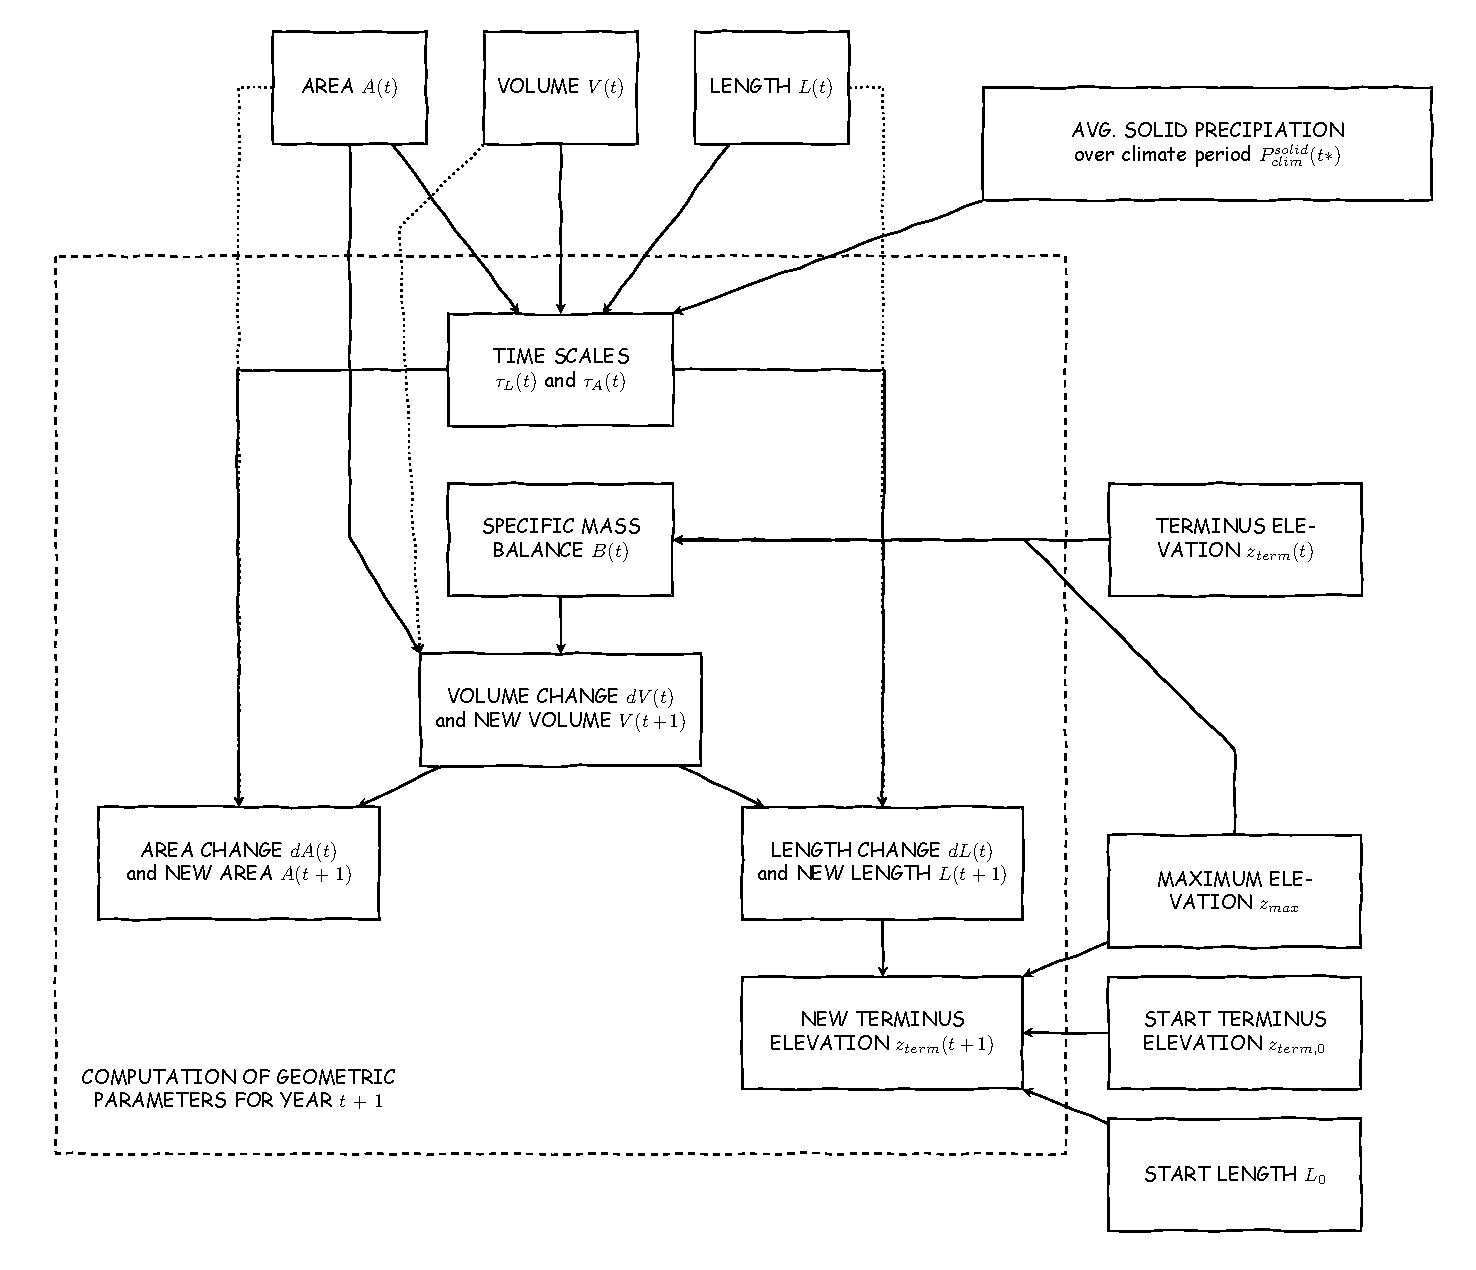
\includegraphics[width=\textwidth]{../flowchart/iterations/scaling.pdf}
            \caption{Schematic of the glacier evolution model's time stepping.}
            \label{fig:iteration-scheme}
        \end{figure}
    
    % subsection glacier_evolution_model (end)

% section general_concepts (end)

% ==== SECTION 2 ===============================================================
\section{Implementation} % (fold)
\label{sec:implementation}

    The \vas{} model is implemented in \href{https://www.python.org/}{Python 3}, following the code structure of the OGGM \citep{Maussion2019}. This compatibility is imperative, since the \vas{} model is no standalone project and relies on the OGGM for data downloads, preprocessing, post processing, and also the same boundary conditions. The mass balance models and the glacier evolution model are implemented as classes with their respective methods. Functions outside these classes can be characterized either as entity tasks, which are applied on individual glaciers, or as global tasks, which run on a population of glaciers that need to share information between each other (mostly for calibration and validation). The entire code can be found on GitHub \url{https://github.com/OGGM/oggm-vas} under an open source license, the following section can be seen as documentation.

    \subsection{Mass balance models} % (fold)
    \label{sub:mass_balance_models_implementation}

        Following the OGGM, the mass balance models are implemented as classes. The \lstinline`VAScalingMassBalance` model handles past or future climate data, while the \lstinline`ConstantVASMassBalance` model and the \lstinline`RandomVASMassBalance` model simulate a constant climate with and without inter-annual variability, respectively.

        \subsubsection{Volume/area scaling mass balance model} % (fold)
        \label{ssub:volume_area_scaling_mass_balance_model_implementation}

            The \lstinline`VAScalingMassBalance` model is the implementation of the original mass balance model by \citet{Marzeion2012b}. The model computes the mass balance of a glacier using historic or projected climate data provided by the climate input file. The general concept is fairly similar to the \lstinline`oggm.core.massbalance.PastMassBalance` model. The main difference is, that the \vas{} mass balance model returns only one average value of glacier-wide mass balance, instead of point mass balance values for the different elevation bands.

            The mass balance model is initialized for a single glacier, denoted by the OGGM specific glacier directory \lstinline`gdir`. Per default, the model will use the calibrated mass balance parameters \mustar{} and \bias{} and read temperature and precipitation records from the preprocessed climate file \lstinline`climate_historical`. An alternative climate file can be used, by supplying either the filename and/or its suffix via the parameters \lstinline`filename` and \lstinline`input_filesuffix`, respectively. It is possible to specify the start year and end year of the climate period (\lstinline`ys` and \lstinline`ye`), if not all available data should be used. The parameter \lstinline`repeat` controls whether the climate period given by \lstinline`[ys, ye]` should be repeated indefinitely in a circular way.

            The \vas{} mass balance model inherits the following methods from the \lstinline`oggm.core.massbalance.MassBalanceModel` super class:
            \begin{itemize}
                \item \lstinline`get_annual_climate()` and \lstinline`get_monthly_climate()` compute and return the mass balance relevant climate information, i.e. positive air temperature at the terminus elevation in [\si{\celsius}] and solid precipitation amount in [\si{\kg\per\square\m}], for the given year and month/year combination, respectively.
                \item \lstinline`get_annual_mb()` and \lstinline`get_monthly_mb()` compute and return the glacier wide average mass balance in [\si{\m\per\s}], for the given year and month/year combination, respectively. A possible mass balance residual \bias{} is applied.
                \item \lstinline`get_specific_mb()` and \lstinline`get_monthly_specific_mb()` compute and return the glacier-wide average specific mass balance in [\si{mm w.e.\per yr}], for the given year and month/year combination, respectively. A possible mass balance residual \bias{} is applied.
            \end{itemize}
            All methods need the glacier terminus elevation \lstinline`min_hgt` and the maximal glacier surface elevation \lstinline`max_hgt` as input parameters. The date is supplied via the \lstinline`year` parameter, using the hydrological float year convention. Given that the scaling mass balance model computes the glacier-wide average mass balance, it is not possible to estimate the equilibrium line altitude. Hence, the the method \lstinline`get_ela()` is not implemented, in contrast to the \lstinline`PastMassBalance` model.
        
        % subsubsection volume_area_scaling_mass_balance_model_implementation (end)

        \subsubsection{Constant climate scenario} % (fold)
        \label{ssub:constant_climate_scenario_implementation}
            The \lstinline`ConstantVASMassBalance` model simulates a constant climate based on the observations averaged over a 31-year period centered on a given year \lstinline`y0`. Hence, the specific mass balance does not change from year to year. The task \lstinline`run_constant_climate(gdir, ...)` initializes a \lstinline`ConstantMassBalance` for the given glacier \lstinline`gdir` and runs for a given number of years \lstinline`nyears`. The task takes an additional temperature bias as parameters \lstinline`temp_bias`, to alter the observed climate records.

            The same idea of a constant climate is used during the mass balance calibration, solving the mass balance equation (Equation~\ref{eq:mass-balance}) for the temperature sensitivity \mustar. So per definition, \mustar{} is the temperature sensitivity to keep the glacier in equilibrium over the 31-year climate period centered around the \textit{equilibrium year} \tstar{}, while neglecting a potential mass balance residual \bias. Consequentially, a \lstinline`ConstantMassBalance` model with \lstinline`y0` = \tstar{} and \bias{} = 0 keeps the glacier in equilibrium.
        
        % subsubsection constant_climate_scenario_implementation (end)

        \subsubsection{Random climate scenario} % (fold)
        \label{ssub:random_climate_scenario_implementation}

            Similar to the \lstinline`ConstantVASMassBalance` model, the \lstinline`RandomVASMassBalance` model is based on a 31-year period centered on a given year \lstinline`y0`. However, the mass balance years are randomly shuffled within that period. More precisely, for each simulated year the model computes the specific mass balance using temperature and precipitation records from a randomly selected year within the given period. Hence, the model runs on a synthetic random climate scenario based on actual observations. A seed \lstinline`seed` for the random generator can be supplied as parameter, to allow for reproducibility. Additionally, it is possible to choose between draws with and without replacement via the \lstinline`unique_sample` parameter.

            The task \lstinline`run_random_climate(gdir, ...)` works analogously to the task \lstinline`run_constant_climate(gdir, ...)`, using an instance of \lstinline`RandomMassBalance` model instead of the \lstinline`ConstantMassBalance` model. Hence, using the climatological period centered around \lstinline`y0` = \tstar, the model glacier should stay in an equilibrium state while underlying minor fluctuations. Supplying a positive or negative temperature bias will result in a retreating or advancing model glacier, respectively, before reaching a new equilibrium after some years.
        
        % subsubsection random_climate_scenario_implementation (end)
    
    % subsection mass_balance_models_implementation (end)

    \subsection{Glacier evolution model} % (fold)
    \label{sub:glacier_evolution_model_implementation}

        The \lstinline`oggm-vas.VAScalingModel` is the implementation of the above describe glacier evolution model (see Section~\ref{sub:glacier_evolution_model}, cf. \citet{Marzeion2012b}) into the OGGM framework.

        An instance of the \lstinline`oggm-vas.VAScalingModel` class is initialized with the initial area \lstinline`area_m2_0`, the initial glacier terminus elevation \lstinline`min_hgt` and maximum glacier surface elevation \lstinline`max_hgt` and an instance of a mass balance model. Additionally, the start year of the simulation \lstinline`year_0` must be defined. Those initial values are stored as instance variables, since they are needed for later computations. Other than that, the \lstinline`oggm-vas.VAScalingModel` object stores all model parameters as instance variables for the year it is in. This includes glacier geometries ($V$, $A$, $L$, $z_\text{min}$, $z_\text{max}$) and their changes ($\Delta V$, $\Delta A$, $\Delta L$), time scales ($\tau_A$, $\tau_L$), the mass balance model and the specific mass balance $B$, but also constants like the scaling parameters ($c_A$, $\gamma$, $c_L$, $q$) and ice density $\rho_\text{ice}$.

        To advance the glacier model, there are three different methods. The \lstinline`step()` method advances the model by one year, following the above described steps (see Section~\ref{sub:glacier_evolution_model}). The method \lstinline`run_until(year_end)` runs the model until the specified year and returns the geometric glacier parameters at the end of the model evolution (year, length, area, volume, terminus elevation and specific mass balance). Thereby, the model starts from whatever year it currently is in. It is possible to start the model run from \lstinline`year_0` with the flag \lstinline`reset`. The method \lstinline`run_until_and_store()` works analogous to the previous one, with the difference that all parameters are stored for each time step (i.e., for each year). The resulting data set is returned and possibly stored to file, if a file path is give. The method \lstinline`run_until_equilibrium()` tries to run the glacier model until an equilibrium state is reached. The model runs for a fixed number of iterations \lstinline`max_ite`, the total elapsed time changes with the chosen time step \lstinline`ystep`. The iteration breaks, either if the glacier volume is below \SI{1}{\cubic\meter} or an equilibrium is reached. An equilibrium state is reached, if the volume change rate $|V(t) - V(t+\Delta t)|/V(t)$ falls below a given value \lstinline`rate`. Therefore, the method should only be used with a \hyperref[ssub:constant_climate_scenario_implementation]{constant climate scenario} (see Section~\ref{sub:mass_balance_models_implementation}).
    
    % subsection glacier_evolution_model_implementation (end)

% section implementation (end)